\documentclass[a4paper, 12pt]{article}

\usepackage{forloop}
\usepackage{graphicx}
\usepackage{subcaption}
\usepackage{amsmath}

\author{Thorvald M. Ballestad}
\title{Assignment 1 - TFY4235\\
  Fractal drum}

\begin{document}
\maketitle

\section{Generating the fractal}
The generation of the fractal structure is implementet quite naievly.
For example, the array of points is not pre-allocated, but appended during each loop-cycle.
The number of points for a given level is easy to calculate, so this would be a simple thing to fix, but as it is not time consuming at all, I have kept the naive method.\\

The fractal points are stored as integers.
The fractal is generated in such a way that the shortest segment is of length one, except when the lattice constatn is increased.
See \ref{sec:lattice}.

\begin{figure}[h]
  \centering
  \begin{subfigure}[b]{.49\textwidth}
      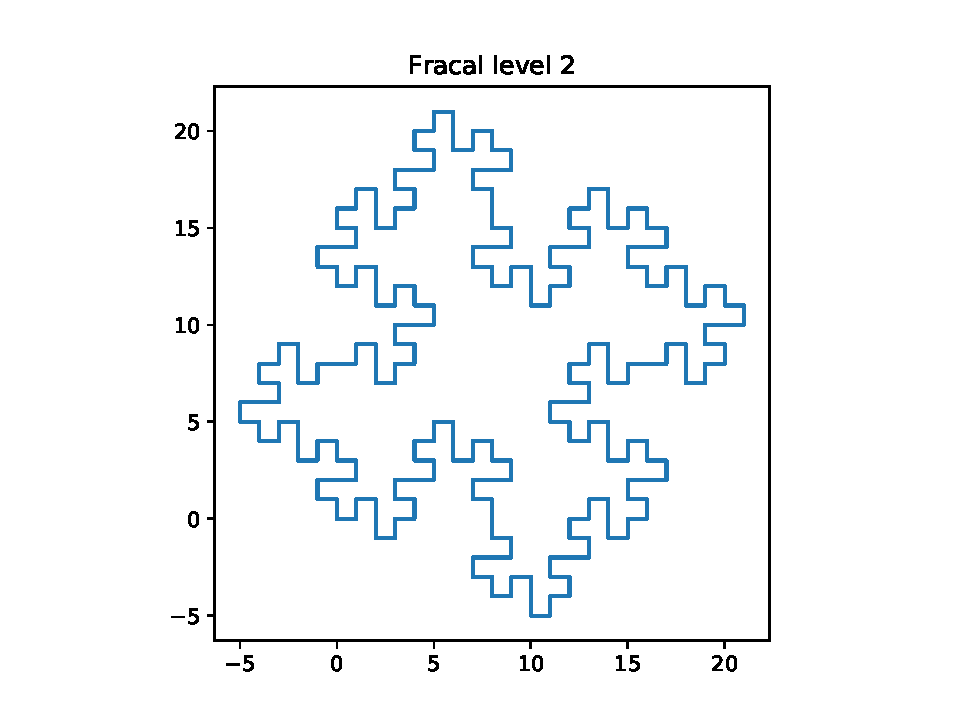
\includegraphics[width=\textwidth]{media/fractal_l2}
  \end{subfigure}
  \begin{subfigure}[b]{.49\textwidth}
      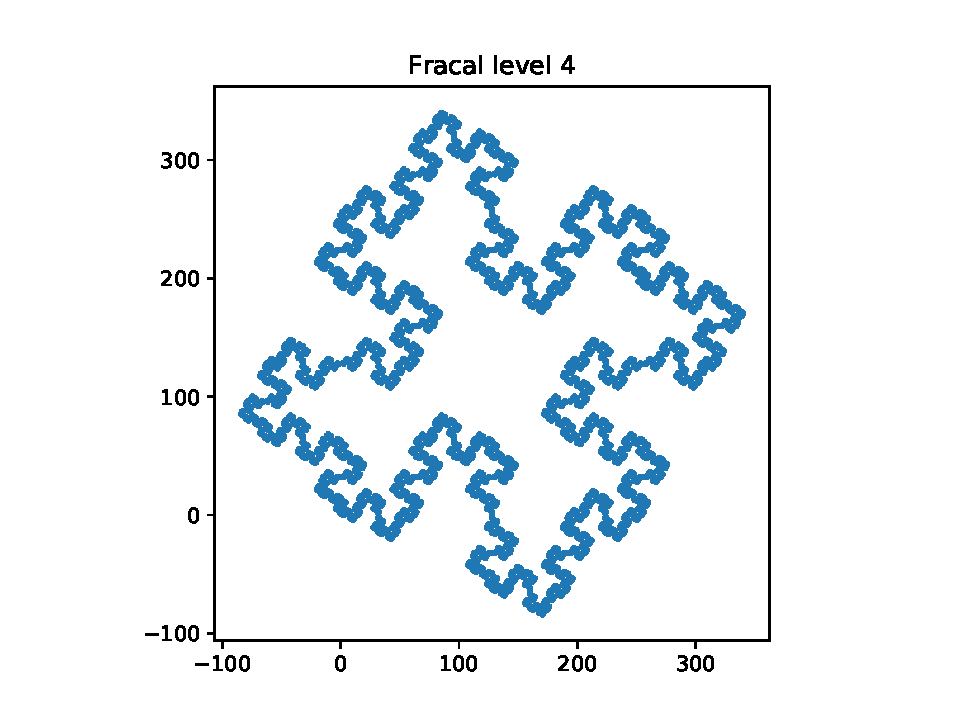
\includegraphics[width=\textwidth]{media/fractal_l4}
  \end{subfigure}
  \caption{Fractal for $l=2$ and $l=4$.}
\end{figure}

\section{The lattice\label{sec:lattice}}
The lattice is a 2D array of integers.
Each array element has a value that corresponds to either inside, outside, or on the border of the fractal.
The lattice constant $\delta$ is implemented in such a way that the shortest segment on the fractal, correspond to $\delta$ steps on the lattice.
Ie. if $\delta=1$, there are no points on the lattice between the start and end point of the line segment on the fractal.

\section{Inside or outside?}
There are two methods implemented in the program for determining if a point is inside or outside the fractal.
The only assumption about the structure that the methods makes, is that every line segment is either vertical or horizonal, and not diagonal.

The first method is a breadth first-type search.
Given a point that we know is inside the structure, add its four cardinal points -- above, below, right, and left -- into a list.
Visit each of the points in the list.
For each of these points that are not border points, append their cardinal points to the list.
Continue this process until the list is empty.
Notice that the list is processed FILO.
A FIFO process would give a depth first search.
One could argue that this method is not complete, as it requires one starting point inside the structure.
However, if one hits the ``edge'' of ones region, without hitting a border point, one knows that the starting point was not inside the structure, and thus the method is complete.
Also, in the problem at hand we know trivially that the center point of our area is inside the curve.
This method will be called middle out.

The second method is based on counting border crossings.
For each point in our area, move in one direction, here left, and count the number of border crossings before reaching the end of the area.
If it is odd, the point is inside, if it is even the point is outside.
The complication is how to count border crossings for a discretized curve.
Here, it is done as follows:
The grid constant must be at least two.
Without this, the problem is not solvable -- one can easily construct cases where it would be ambiguous where the curve goes.
When scanning, in this case left, check for each point if it is a border point.
If it is, check if the point below it is also a border point.
If that is the case, count it as a border crossing.
This method will be called scan.

On a level 4 fractal with grid constant 2, the two methods performed as follows:
\begin{table}
  \centering
\begin{tabular}{lrrr}
  Method& Time[s]& Allocations& Memory[MiB]\\
  \hline
  Middle out& 0.069& 788K& 32\\
  Scan& 3.33& 54M& 835
\end{tabular}
\caption{Performance of methods for determining if points are inside or outside.}
\end{table}

\section{Calculation eigenmodes}
We want to solve
\begin{subequations}
  \label{eq:helm}
  \begin{align}
    -\nabla^2 U(x, \omega) &= \frac{\omega^2}{v^2} U(x, \omega), &&\text{in } \Omega\\
    U(x, \omega) &= 0, &&\text{on } \partial \Omega.
  \end{align}
\end{subequations}

We will use the five point stencil for $\nabla^2$.
$$
h^2\nabla^2 U \approx U(x+h, y) + U(x-h, y) + U(x, y+h) + U(x, y-h) - 4U(x,y). 
$$

We convert \eqref{eq:helm} into an eigenproblem on matrix form.
This is done by creating a 1D array $U$ containing all the innner points of the fractal.
A corresponding matrix, representing $\nabla^2$ with the five point stencil is also made.
The programatic challenge here is constructing the matrix, or more precisely mapping our structure onto $U$, and then finding which entries in our eigenmatrix corresponds to the correct point.

There are two aspects of the solution worth mentioning.
When discussing the lattice, it was mentioned that each point is an integer representing either inside, outside or border.
More specifically negative one represents outside and zero border.
Any positive integer is inside.
Each inner point is given an unique positive integer, representing that points position in $U$.
This way, we have a direct lookup from the grid to $U$.
By also creating an array of inner points, ie. an array of tuples containing the coordinates to that point in the array, we have a direct lookup also the other way.\\

The second aspect worth mentioning is how we store the eigenmatrix.
This matrix is mainly zeros, therefore we store it in compressed sparse column format, which is the standard sparse format in Julia.

\newcounter{mode}
\forloop{mode}{1}{\value{mode}<10}{
  \begin{figure}[p]
    \centering
    \begin{subfigure}[b]{.49\textwidth}
      \includegraphics[width=\textwidth]{media/modes/mode_\arabic{mode}.pdf}
    \end{subfigure}
    \stepcounter{mode}
    \begin{subfigure}[b]{.49\textwidth}
      \includegraphics[width=\textwidth]{media/modes/mode_\arabic{mode}.pdf}
    \end{subfigure}
  \end{figure}
}


\begin{table}
  \centering
  \begin{tabular}{ll}
    \#& $\omega/v$\\
    \hline
    1&	1.501E-04\\
    2&	3.370E-04\\
    3&	3.370E-04\\
    4&	3.501E-04\\
    5&	3.539E-04\\
    6&	3.840E-04\\
    7&	3.840E-04\\
    8&	5.260E-04\\
    9&	6.031E-04\\
    10&	6.384E-04
  \end{tabular}
  \caption{The 10 lowest eigenfrequencies, calculated at $l=??$ and with lattice constant ??. TODO fill out values}
\end{table}
\end{document}
